82. $\cfrac{(2x^2+7x-4)(x-3)^2}{x+6}\leqslant0\Leftrightarrow\cfrac{(2x-1)(x+4)(x-3)^2}{x+6}\leqslant0.$
Применив метод интервалов, найдём ответ:
\begin{figure}[ht!]
\center{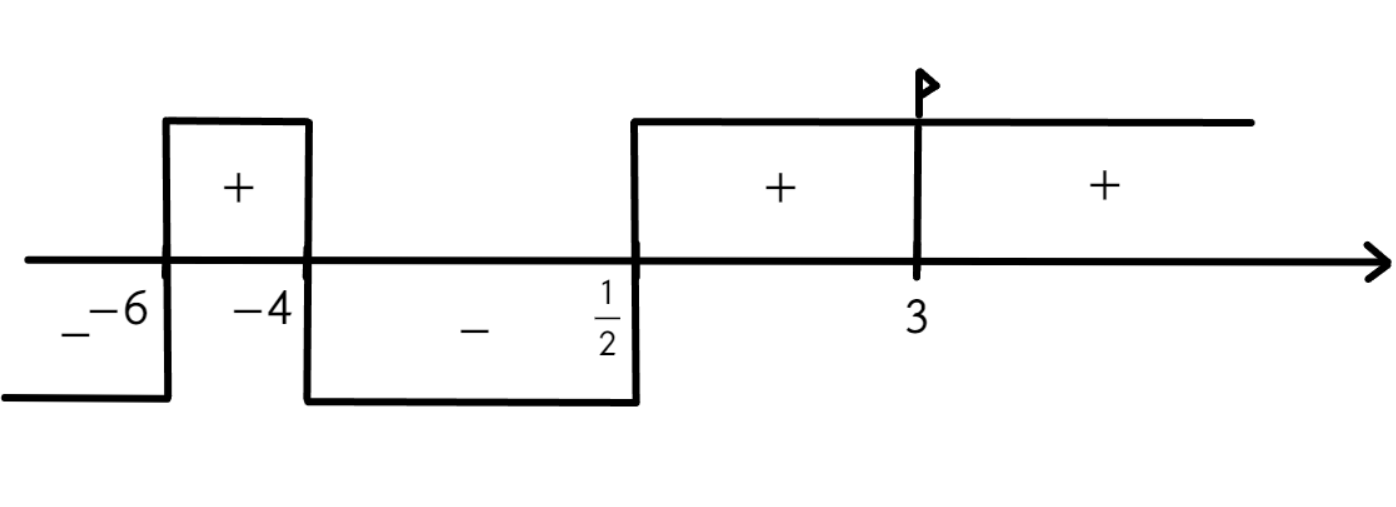
\includegraphics[scale=0.35]{int82.png}}
\end{figure}
$x\in(-\infty;-6)\cup\left[-4;\cfrac{1}{2}\right]\cup\{3\}.$\newpage\noindent
